\subsection{The Cross Product}

\begin{center}
\begin{tikzpicture}
\coordinate (O) at (0,0);
\coordinate (A) at (3.5,0);
\coordinate (B) at (1.5,1.2);
\coordinate (C) at (0,3);
% vectors
\draw[->, thick] (O) -- (A) node[below right]{$\mathbf{A}$};
\draw[->, thick] (O) -- (B) node[above right]{$\mathbf{B}$};
\draw[->, thick] (O) -- (C) node[left]{$\mathbf{C}=\mathbf{A}\times\mathbf{B}$};
% angle
\draw (0.8,0) arc[start angle=0, end angle=39, radius=0.8]
    node[midway, right]{\small$\theta$};
% dashed parallelogram
\draw[dashed] (A) -- ++(1.5,1.2) -- (B);
\end{tikzpicture}
\end{center}

\[
    \lVert\mathbf{A}\times\mathbf{B}\rVert
    = \lVert\mathbf{A}\rVert\,\lVert\mathbf{B}\rVert\sin\theta
    \quad\longrightarrow\quad \text{Area of parallelogram}
\]

$\mathbf{A}\times\mathbf{B} = \mathbf{0}
\;\Longleftrightarrow\;
\mathbf{A}=\mathbf{0},\;\mathbf{B}=\mathbf{0},\;\text{or } \mathbf{A}\parallel\mathbf{B}$

\subsubsection*{Formula}

\[
    \mathbf{A}\times\mathbf{B}
    = \begin{pmatrix}
        A_{2}B_{3}-A_{3}B_{2} \\
        A_{3}B_{1}-A_{1}B_{3} \\
        A_{1}B_{2}-A_{2}B_{1}
      \end{pmatrix}
\]

\subsubsection*{Scalar Triple Product}

\[
    (\mathbf{A}\times\mathbf{B})\cdot\mathbf{C}
    = \lVert\mathbf{A}\times\mathbf{B}\rVert\;\text{comp}_{\mathbf{A}\times\mathbf{B}}\,\mathbf{C}
    \quad\longrightarrow\quad \text{Volume of parallelepiped}
\]

\begin{center}
\begin{tikzpicture}
\coordinate (O) at (0,0);
\coordinate (A) at (3.5,0);
\coordinate (B) at (1.2,1);
\coordinate (C) at (0.8,2.8);
\coordinate (AB) at ($(A)+(B)$);
\coordinate (AC) at ($(A)+(C)$);
\coordinate (BC) at ($(B)+(C)$);
\coordinate (ABC) at ($(A)+(B)+(C)$);
% bottom face
\draw[->, thick] (O) -- (A) node[below right]{$\mathbf{A}$};
\draw[->, thick] (O) -- (B) node[above left]{$\mathbf{B}$};
\draw[thick] (A) -- (AB) -- (B);
% top face
\draw[dashed] (C) -- (AC);
\draw[dashed] (C) -- (BC);
\draw[thick] (AC) -- (ABC) -- (BC);
% vertical edges
\draw[->, thick] (O) -- (C) node[left]{$\mathbf{C}$};
\draw[thick] (A) -- (AC);
\draw[thick] (B) -- (BC);
\draw[dashed] (AB) -- (ABC);
% A x B arrow
\coordinate (N) at ($(O)!0.5!(AB) + (0,2.5)$);
\draw[->, thick, densely dotted] ($(O)!0.5!(AB)$) -- (N)
    node[right]{$\text{comp}_{\mathbf{A}\times\mathbf{B}}\,\mathbf{C}$};
\end{tikzpicture}
\end{center}

\subsection{Equations of Lines and Planes}

\subsubsection*{Lines}

\begin{example}
Line through $\mathbf{P}=\ve{1,\,3}$ and $\mathbf{Q}=\ve{7,\,-1}$:

\begin{center}
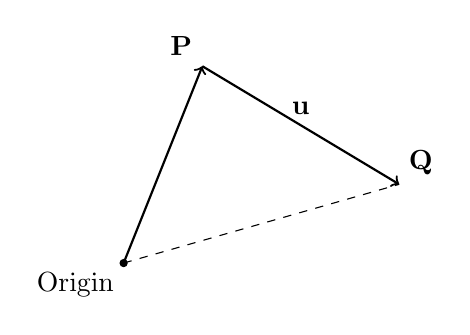
\begin{tikzpicture}
\coordinate (O) at (0,0);
\coordinate (P) at (1,2.5);
\coordinate (Q) at (3.5,1);
\draw[->, thick] (O) -- (P) node[above left]{$\mathbf{P}$};
\draw[->, thick] (P) -- (Q) node[midway, above]{$\mathbf{u}$};
\draw[dashed] (O) -- (Q) node[above right]{$\mathbf{Q}$};
\fill (O) circle(1.5pt) node[below left]{Origin};
\end{tikzpicture}
\end{center}

$\mathbf{u} = \vec{PQ} = \mathbf{Q}-\mathbf{P} = \ve{6,\,-4}$

All points on $\overline{PQ}$: \;
$\mathbf{P} + t\,\mathbf{u} = \ve{1+6t,\; 3-4t}$, \; $t\in\R$.
\end{example}

For point vectors $\mathbf{r}_{1},\,\mathbf{r}_{2}$, all points on the line $\mathbf{r}_{1}$--$\mathbf{r}_{2}$:
\[
    \mathbf{r}(t) = \mathbf{r}_{1} + t(\mathbf{r}_{2}-\mathbf{r}_{1}), \quad t\in\R
\]

Let $\mathbf{r}_{1}=\ve{x_{1},y_{1},z_{1}}$,
$\mathbf{r}_{2}-\mathbf{r}_{1}=\ve{a,b,c}$.
Then $\mathbf{r}(t)=\ve{x,y,z}$ gives the symmetric equations:
\[
    \frac{x-x_{1}}{a} = \frac{y-y_{1}}{b} = \frac{z-z_{1}}{c} = t
\]

\subsubsection*{Planes}

\begin{definition}[Plane]
A plane through $\mathbf{r}_{0}$, perpendicular to normal $\mathbf{n}$:

\begin{center}
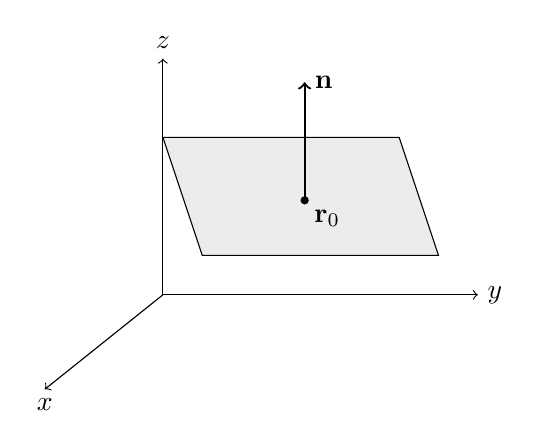
\begin{tikzpicture}
% axes
\draw[->] (0,0) -- (-1.5,-1.2) node[below]{$x$};
\draw[->] (0,0) -- (4,0) node[right]{$y$};
\draw[->] (0,0) -- (0,3) node[above]{$z$};
% plane (parallelogram)
\fill[gray!15] (0.5,0.5) -- (3.5,0.5) -- (3,2) -- (0,2) -- cycle;
\draw (0.5,0.5) -- (3.5,0.5) -- (3,2) -- (0,2) -- cycle;
% r0 and n
\coordinate (R) at (1.8,1.2);
\fill (R) circle(1.5pt) node[below right]{$\mathbf{r}_{0}$};
\draw[->, thick] (R) -- ++(0,1.5) node[right]{$\mathbf{n}$};
\end{tikzpicture}
\end{center}

Equation: $(\mathbf{v}-\mathbf{r}_{0})\cdot\mathbf{n} = 0$,
where $\mathbf{v}$ is on the plane.

Also: $\mathbf{v}\cdot\mathbf{n} = k = \mathbf{r}_{0}\cdot\mathbf{n}$ (constant).

Also in the form $ax+by+cz = k$,
where $\mathbf{v}=\ve{x,y,z}$, $\mathbf{n}=\ve{a,b,c}$.
\end{definition}

\begin{example}
Find the plane through $P(1,0,0)$, $Q(0,2,0)$, $R(0,0,3)$.

$\mathbf{u} = \vec{PQ} = \ve{-1,\,2,\,0}$, \quad
$\mathbf{v} = \vec{PR} = \ve{-1,\,0,\,3}$

$\mathbf{n} = \mathbf{u}\times\mathbf{v} = \ve{6,\,3,\,2}$

Equation: $(\mathbf{v}-\mathbf{P})\cdot\mathbf{n}=0
\;\Longrightarrow\; 6x+3y+2z = 6$
\end{example}

\subsubsection*{Intersection of Two Planes}

Planes with normals $\mathbf{n}_{1}$, $\mathbf{n}_{2}$:
$\mathbf{n}_{1}\parallel\mathbf{n}_{2} \Longrightarrow$ same or parallel planes.
Otherwise they intersect in a line.

\begin{example}
$\begin{cases} x+y+z=2 \\ x-z=1 \end{cases}$ --- find the line of intersection.

\begin{enumerate}
    \item Get a point $P$: let $z=0$, then $x=1$, $y=1$.
          So $P=(1,1,0)$.
    \item Get direction $\mathbf{v}$:
          $\mathbf{v}\perp\mathbf{n}_{1}=\ve{1,1,1}$ and
          $\mathbf{v}\perp\mathbf{n}_{2}=\ve{1,0,-1}$, so
          \[
              \mathbf{v} = \mathbf{n}_{1}\times\mathbf{n}_{2}
              = \ve{-1,\,2,\,-1}
          \]
\end{enumerate}

Line: $\mathbf{r}(t) = P + \mathbf{v}\,t$, \; $t\in\R$.
\end{example}

\subsection{Quadric Surfaces}

\begin{example}
Identify $x^{2}+4x-2y^{2}+3z^{2}-6z=1$.

Complete the square:
\[
    (x+2)^{2}-2y^{2}+3(z-1)^{2}=8
\]
Let $X=x+2$, $Y=y$, $Z=z-1$:
\[
    X^{2}-2Y^{2}+3Z^{2}=8
\]

Cross sections:
\begin{itemize}[nosep]
    \item $X=\text{const}$: $2Y^{2}-3Z^{2}=X^{2}-8$ --- hyperbola
          (asymptotes $2Y^{2}=3Z^{2}$)
    \item $Y=\text{const}$: $X^{2}+3Z^{2}=8+2Y^{2}$ --- ellipse
    \item $Z=\text{const}$: $X^{2}-2Y^{2}=8-3Z^{2}$ --- hyperbola
\end{itemize}
\end{example}
